% ============================================================
%  Chapter 7 – Stochastic Optimization
%  Lectures on Monte Carlo Theory – Leskelä & Vihola
% ============================================================
\documentclass[aspectratio=169,10pt]{beamer}
\usetheme{Madrid}
\usecolortheme{seahorse}
\setbeamertemplate{footline}[frame number]

% ── packages ────────────────────────────────────────────────
\usepackage{amsmath,amssymb,mathtools}
\usepackage{bm}
\usepackage{graphicx}
\usepackage{booktabs}
\usepackage{listings}
\usepackage{xcolor}
\usepackage{algorithm}
\usepackage{algpseudocode}
\usepackage{tikz}

\graphicspath{{figures/}}

% ── listings style ──────────────────────────────────────────
\lstdefinestyle{python}{
  language=Python,
  basicstyle=\ttfamily\scriptsize,
  numbers=left,
  numberstyle=\tiny\color{gray},
  frame=single,
  backgroundcolor=\color{gray!7},
  keywordstyle=\color{blue!70!black}\bfseries,
  commentstyle=\color{green!50!black}\itshape,
  stringstyle=\color{orange!80!black},
  breaklines=true,
  showstringspaces=false,
  tabsize=4,
}

% ── macros ──────────────────────────────────────────────────
\newcommand{\R}{\mathbb{R}}
\newcommand{\E}{\mathbb{E}}
\newcommand{\Prob}{\mathbb{P}}
\newcommand{\bx}{\mathbf{x}}
\newcommand{\bv}{\mathbf{v}}
\newcommand{\bw}{\mathbf{w}}
\newcommand{\btheta}{\boldsymbol{\theta}}
\newcommand{\calS}{\mathcal{S}}

% ============================================================
\title[Ch.7 Stochastic Optimization]{Chapter 7\\Stochastic Optimization}
\subtitle{Lectures on Monte Carlo Theory}
\author{Leskel\"{a} \& Vihola}
\date{}
% ============================================================

\begin{document}

% ── Title ───────────────────────────────────────────────────
\begin{frame}
  \titlepage
\end{frame}

% ── Outline ─────────────────────────────────────────────────
\begin{frame}{Chapter Outline}
  \tableofcontents
\end{frame}

% ============================================================
\section{Introduction}
% ============================================================

\begin{frame}{The Stochastic Optimization Problem}
  \textbf{Goal.}  Given a function $h : \calS \to \R$, find

  \begin{block}{Optimization Objective}
    \[
      \gamma^{\mathrm{opt}} = \max_{x \in \calS} h(x),
      \qquad
      x^{\mathrm{opt}} = \arg\max_{x \in \calS} h(x).
    \]
    \begin{itemize}
      \item $\calS$ -- state / solution space (may be combinatorial)
      \item $h$ -- objective / performance function (to be \emph{maximized})
      \item Equivalently minimize cost $H = -h$
    \end{itemize}
  \end{block}

  \medskip
  \textbf{Core idea (Monte Carlo approach):} construct a Markov chain
  whose stationary distribution $\pi$ puts high probability on good
  solutions, then sample from it.

  \medskip
  \textbf{Methods covered:}
  \begin{enumerate}
    \item Metropolis / Gibbs at fixed temperature
    \item Simulated Annealing (decreasing temperature)
    \item Locally Informed Proposals (gradient-aware)
    \item Cross-Entropy (CE) method
    \item Metropolis–CE hybrid
  \end{enumerate}
\end{frame}

\begin{frame}{Running Examples Throughout the Chapter}
  Two combinatorial problems are used as benchmarks:
  \medskip

  \begin{columns}[T]
    \column{0.48\textwidth}
    \begin{block}{Travelling Salesman Problem (TSP)}
      \begin{itemize}
        \item $n$ cities, symmetric distance matrix $\mathbf{M}$
        \item Find permutation $\sigma^* \in S_n$ minimising total distance
          \[l(\sigma) = \sum_{k=1}^{n-1}\mathbf{M}(\sigma(k),\sigma(k+1))
            + \mathbf{M}(\sigma(n),\sigma(1))\]
        \item NP-hard; optimal for $n=13$ is \textbf{7024} (Held-Karp)
      \end{itemize}
    \end{block}

    \column{0.48\textwidth}
    \begin{block}{0-1 Knapsack Problem}
      \begin{itemize}
        \item $d$ items, weights $\bw$, values $\bv$, capacity $W$
        \item Find $\bx \in \{0,1\}^d$ maximising $\bv \cdot \bx$
          subject to $\bw \cdot \bx \le W$
        \item Simulation: $d=100$, $w_i=i$, $v_i=i^{1.2}$, $W=3000$
      \end{itemize}
    \end{block}
  \end{columns}
\end{frame}

% ============================================================
\section{7.1 Metropolis and Gibbs Based Methods}
% ============================================================

\begin{frame}{7.1 Metropolis and Gibbs Based Methods}
  \textbf{Setting.}  Graph $G=(V,E)$, cost $H:V\to\R_+$.
  Want to find $\arg\min_v H(v)$.

  \begin{block}{Boltzmann Distribution (Eq.~7.1.1)}
    \[
      \pi^T_v = \frac{e^{-H(v)/T}}{\displaystyle\sum_{v' \in V} e^{-H(v')/T}},
      \qquad v \in V, \quad T > 0.
    \]
    \begin{itemize}
      \item $T$ -- \emph{temperature} parameter
      \item As $T \to 0$: mass concentrates on minimisers of $H$
      \item As $T \to \infty$: approaches uniform distribution
      \item Key identity: $\arg\min_v H(v) = \arg\max_v \pi^T_v$
    \end{itemize}
  \end{block}

  \medskip
  To maximise $f: V \to \R_+$, set $H(v) = -f(v)$.
\end{frame}

\begin{frame}{Boltzmann Distribution at Different Temperatures}
  \begin{center}
    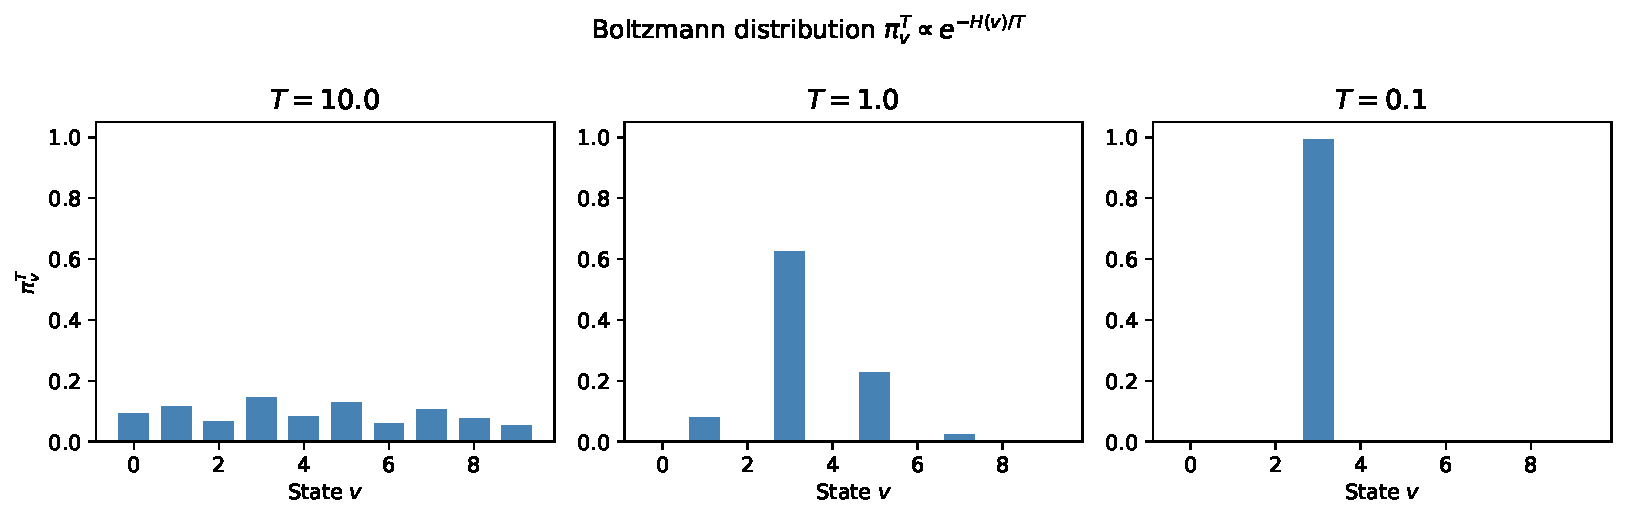
\includegraphics[width=0.88\textwidth]{fig_boltzmann}
  \end{center}
  \small
  As $T$ decreases, the Boltzmann distribution concentrates mass on the
  minimiser of $H$ (the state with smallest cost).
\end{frame}

\begin{frame}{Acceptance Probability for Metropolis on Graph}
  Use the \textbf{random walk} on $G$ as proposal matrix $\mathbf{Q}$.
  The Metropolis acceptance probability is:

  \begin{block}{Acceptance Probability (Algorithm 61)}
    \[
      \alpha^T_{vv'} = \min\!\left(1,\;
        \frac{\deg(v)}{\deg(v')}\,
        e^{(H(v)-H(v'))/T}
      \right),
      \qquad v,v' \in V.
    \]
    \[
      p^T_{vv'} = \frac{1}{\deg(v)}\min\!\left(1,\;
        \frac{\deg(v)}{\deg(v')}\,
        e^{(H(v)-H(v'))/T}
      \right), \quad q_{vv'}>0.
    \]
  \end{block}
  \begin{itemize}
    \item $\deg(v)$ -- degree of vertex $v$ in $G$
    \item Moves to a \emph{worse} solution ($H(v')>H(v)$) with positive prob
    \item This allows escape from local minima
  \end{itemize}
\end{frame}



\begin{frame}[fragile]{Algorithm 61: Metropolis for Boltzmann Distribution}
  \begin{lstlisting}[style=python]
import numpy as np

def metropolis_boltzmann_step(v, neighbors, H, T, rng):
    """One step of Metropolis-Hastings for Boltzmann distribution."""
    deg_v  = len(neighbors[v])
    v_prop = rng.choice(neighbors[v])             # propose neighbor uniformly
    deg_vp = len(neighbors[v_prop])
    # Acceptance probability
    alpha = min(1.0,
                (deg_v / deg_vp) * np.exp((H[v] - H[v_prop]) / T))
    U = rng.uniform()
    return v_prop if U <= alpha else v

# Run for n_steps
def run_metropolis(v0, neighbors, H, T, n_steps, seed=0):
    rng   = np.random.RandomState(seed)
    chain = [v0]
    v     = v0
    for _ in range(n_steps):
        v = metropolis_boltzmann_step(v, neighbors, H, T, rng)
        chain.append(v)
    return chain
  \end{lstlisting}
\end{frame}

\begin{frame}{Application: Decrypting a Substitution Cipher}
  \textbf{Setup.} A substitution cipher permutes the alphabet:
  $\sigma: \Sigma \to \Sigma$, $|\Sigma|=26$.
  State space $\calS = S_{26}$ ($26! \approx 4 \times 10^{26}$ permutations).

  \begin{block}{Log-Likelihood Score Function}
    \[
      l(\sigma) = \sum_{i=1}^{L-1} \log \mathbf{M}(\sigma(c_i),\,\sigma(c_{i+1})),
    \]
    where $\mathbf{M}(a,b)$ is the bigram frequency in English text
    (\emph{War and Peace}), and $c_1,\ldots,c_L$ is the ciphertext.
  \end{block}

  \textbf{Boltzmann distribution:}
  $\pi_\sigma = \frac{1}{z} l(\sigma)$ (proportional to likelihood).

  \textbf{Proposal:} swap two uniformly chosen symbols (transposition).

  \medskip
  \textbf{Result:} After 3000 steps the message is essentially decrypted
  (log-likelihood improves from $-4274$ to $-815$).
\end{frame}

\begin{frame}{Metropolis Cipher Decryption: Log-Likelihood Trace}
  \begin{columns}
    \column{0.58\textwidth}
    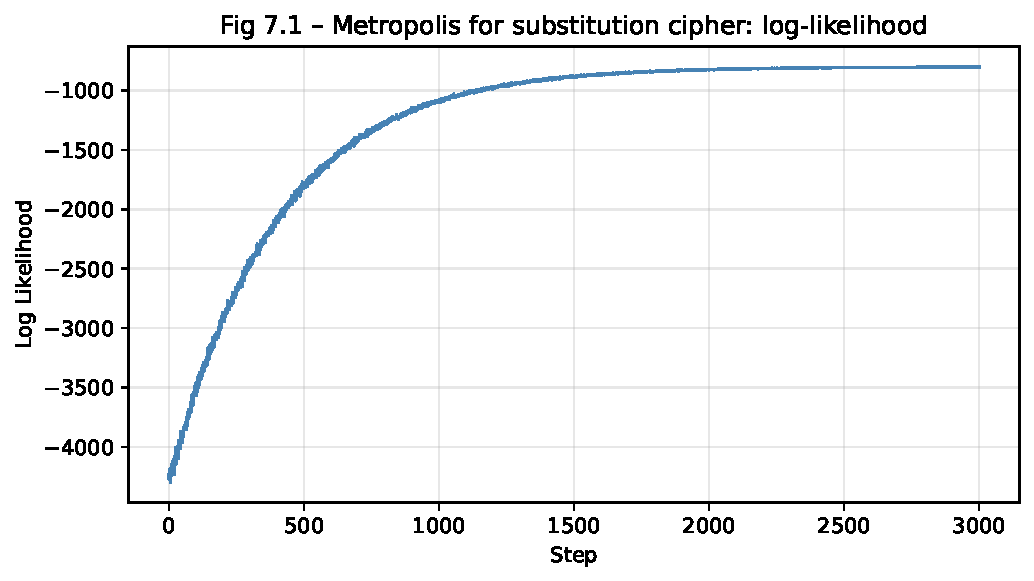
\includegraphics[width=\textwidth]{fig_cipher_loglik}
    \column{0.40\textwidth}
    \small
    \textbf{Table 7.1} (selected steps):\\[4pt]
    \begin{tabular}{r|l|r}
      \toprule
      Step & Decrypted (start) & Log-lik\\
      \midrule
      1    & yckqzchskqhaqyc\ldots & $-4274$\\
      1000 & the whole of that\ldots & $-896$\\
      2000 & \ldots anna skent\ldots  & $-826$\\
      3000 & \ldots anna spent\ldots  & $-815$\\
      \bottomrule
    \end{tabular}\\[6pt]
    Rapid improvement in first 500 steps, then gradual refinement.
  \end{columns}
\end{frame}

\begin{frame}{The 0-1 Knapsack Problem}
  \textbf{Setup.}
  $d$ items, weights $\bw=(w_1,\ldots,w_d)$, values $\bv=(v_1,\ldots,v_d)$.
  Find $\bx \in \{0,1\}^d$ maximising total value subject to capacity $W$.

  \begin{block}{Boltzmann Distribution for Knapsack}
    \[
      \pi_{\bx} =
      \begin{cases}
        \dfrac{\exp(\bv\cdot\bx/T)}{z_T} & \text{if } \bw\cdot\bx \le W,\\[6pt]
        0 & \text{otherwise}.
      \end{cases}
    \]
    States violating the weight constraint have zero probability.
  \end{block}

  \textbf{Gibbs conditional (Algorithm 63):}
  \[
    \Prob(Z(i)=1 \mid Z_{-i}=\bx_{-i})
    = \frac{1}{1+\exp\!\left(-\tfrac{1}{T}v_i x_i\right)}.
  \]
\end{frame}

\begin{frame}[fragile]{Algorithms 63 \& 64: Gibbs and Metropolis for Knapsack}
  \begin{lstlisting}[style=python]
import numpy as np

def gibbs_knapsack_step(x, w, v, W, T, rng):
    """Gibbs sampler step for 0-1 knapsack (Algorithm 63)."""
    d = len(x);  i = rng.randint(0, d)
    x_new = x.copy();  x_new[i] = 1
    if np.dot(w, x_new) > W:
        x_new[i] = 0          # forced: adding item exceeds capacity
    else:
        prob1 = 1.0 / (1.0 + np.exp(-v[i] / T))
        x_new[i] = 1 if rng.rand() <= prob1 else 0
    x[i] = x_new[i];  return x

def metropolis_knapsack_step(x, w, v, W, T, rng):
    """Metropolis step for 0-1 knapsack (Algorithm 64)."""
    d = len(x);  i = rng.randint(0, d)
    x_new = x.copy();  x_new[i] = 1 - x_new[i]   # flip bit i
    if np.dot(w, x_new) <= W:
        alpha = min(1.0, np.exp((1/T) * (1 - 2*x[i]) * v[i]))
    else:
        alpha = 0.0
    if rng.rand() < alpha:
        x[:] = x_new
    return x
  \end{lstlisting}
\end{frame}

\begin{frame}{Knapsack Simulation Results}
  \begin{columns}
    \column{0.58\textwidth}
    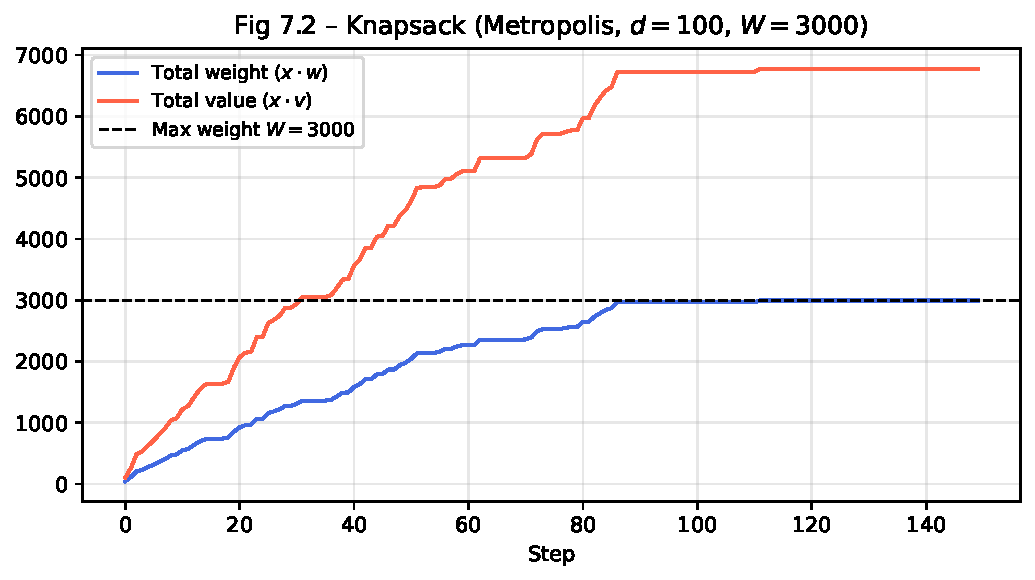
\includegraphics[width=\textwidth]{fig_knapsack_metropolis}
    \column{0.40\textwidth}
    \small
    \textbf{Parameters:}\\
    $d=100$, $W=3000$\\
    $w_i=i$, $v_i=i^{1.2}$, $T=1$\\[6pt]
    After 150 steps:\\
    \begin{itemize}
      \item Total weight $X_{150}\cdot\bw \approx 2977$
      \item Total value $X_{150}\cdot\bv \approx 6745$
    \end{itemize}
    \vspace{4pt}
    The weight stays near capacity $W=3000$ while value climbs steadily.\\[4pt]
    \emph{Remark:} results improve by tuning $T$.
  \end{columns}
\end{frame}

% ============================================================
\section{7.2 Simulated Annealing}
% ============================================================

\begin{frame}{7.2 Simulated Annealing -- Motivation}
  \textbf{Problem with fixed temperature:}
  \begin{itemize}
    \item $T$ large $\Rightarrow$ moves freely, but stationary distribution
      nearly uniform (poor optimiser).
    \item $T$ small $\Rightarrow$ stationary distribution near optimal, but
      chain mixes slowly (gets trapped in local minima).
  \end{itemize}

  \textbf{Key idea (Simulated Annealing):}
  Start with a high temperature $T_0$ and \emph{decrease} it according to
  a \textbf{cooling schedule} $T_0 \ge T_1 \ge \cdots \searrow 0$.

  \begin{block}{Modified Boltzmann (per step $k$)}
    \[
      \pi^{T_k}_v = \frac{\deg(v)\exp(-H(v)/T_k)}{z_{T_k}}, \qquad v \in V.
    \]
    The transition matrix at step $k$ is
    \[
      p_{vv'}(k) = \frac{1}{\deg(v)}\min\!\left(1,\,
        \exp\!\left(-\tfrac{1}{T_k}(H(v')-H(v))\right)\right).
    \]
  \end{block}
\end{frame}

\begin{frame}{Convergence of Simulated Annealing}
  \begin{block}{Proposition 7.2.2 (Convergence at Fixed $T$)}
    For fixed $T_k \equiv T$ the non-homogeneous MC satisfies
    \[
      \lim_{T \searrow 0}\; \lim_{\substack{k\to\infty \\ T_k=T}}
      \Prob(X_k \in D^*) = 1,
    \]
    where $D^* = \{v \in V : H(v) = \min_{v'} H(v')\}$ is the optimal set.
  \end{block}

  \textbf{Cooling schedule constraint:} Let $c = \min_{v' \in \mathcal{N}(v)}(H(v')-H(v))$
  for a local minimum $v$. If
  \[
    \sum_j e^{-c/T_j} < \infty
  \]
  then the chain can \emph{remain} in the local minimum -- cooling is too fast.

  \medskip
  \textbf{Practical guidance:}
  Use $T_k = d\log(k)$ for some $d > 0$ (``logarithmic cooling'').
  This is slow but theoretically justified.
\end{frame}

\begin{frame}{Cooling Schedules}
  \begin{columns}
    \column{0.58\textwidth}
    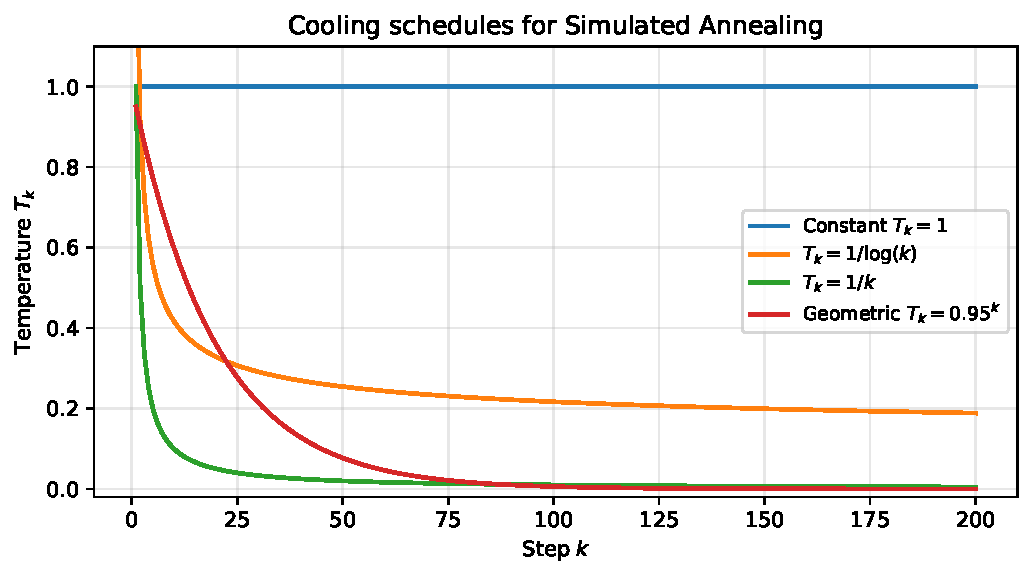
\includegraphics[width=\textwidth]{fig_cooling_schedule}
    \column{0.40\textwidth}
    \small
    Common cooling schedules:\\[6pt]
    \begin{itemize}
      \item \textbf{Constant}: $T_k = T$ (plain Metropolis)
      \item \textbf{Logarithmic}: $T_k = 1/\log(k)$\\
            Theoretically valid, but slow
      \item \textbf{Linear}: $T_k = 1/k$\\
            Too fast -- can trap
      \item \textbf{Geometric}: $T_k = \beta^k$, $\beta < 1$\\
            Popular in practice
    \end{itemize}
    \vspace{4pt}
    Convergence requires $T_k \searrow 0$ \emph{slowly enough}.
  \end{columns}
\end{frame}

\begin{frame}{Non-Homogeneous Markov Chains}
  \textbf{Definition.} A sequence $(Y_n)$ is a
  \textbf{time non-homogeneous Markov chain} on $\calS=\{s_1,\ldots,s_m\}$
  if for any $s_{i_0},\ldots,s_{i_k} \in \calS$:
  \[
    \Prob(Y_0=s_{i_0}, Y_1=s_{i_1},\ldots, Y_k=s_{i_k})
    = \mu_{s_{i_0}} p_{s_{i_0}s_{i_1}}(1) \cdots p_{s_{i_{k-1}}s_{i_k}}(k).
  \]
  The transition probability at step $k$ is $p_{s_is_j}(k) = \Prob(Y_{k+1}=s_j \mid Y_k=s_i)$.

  \begin{block}{Distribution of $Y_l$ (Eq.~7.2.3)}
    \[
      (\Prob(X_l=s_1), \ldots, \Prob(X_l=s_m)) = \bm{\mu}\,\mathbf{P}(0,l),
    \]
    where $\mathbf{P}(k,l) = \mathbf{P}(k)\mathbf{P}(k+1)\cdots\mathbf{P}(l)$.
  \end{block}

  \textbf{Remark 7.2.3.} SA (Algorithm 65) is a non-homogeneous MC with
  $p_{vv'}(k) = q_{vv'}\,\alpha_k$.
\end{frame}

\begin{frame}{Mass Concentration as $T \searrow 0$}
  \begin{columns}
    \column{0.58\textwidth}
    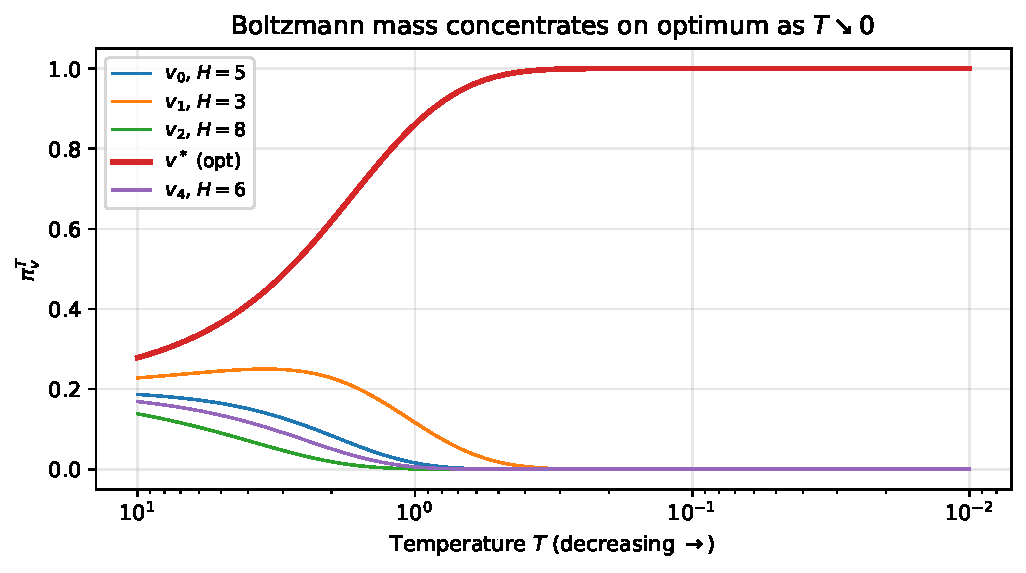
\includegraphics[width=\textwidth]{fig_nonhomogeneous_mc}
    \column{0.40\textwidth}
    \small
    As temperature decreases:\\[6pt]
    \begin{itemize}
      \item All probability mass concentrates on the \textbf{optimal state}
        $v^* = \arg\min H$
      \item States with higher cost $H$ lose mass exponentially fast
      \item Proof: denominator in $\pi^T_v$ dominated by optimal terms
    \end{itemize}
    \vspace{6pt}
    \textbf{This justifies SA}: run at decreasing temperatures to track
    the mass toward the global optimum.
  \end{columns}
\end{frame}

\begin{frame}[fragile]{Algorithm 65: Simulated Annealing (One Step)}
  \begin{lstlisting}[style=python]
def sa_step(v, neighbors, H, T_k, rng):
    """One SA step with temperature T_k (Algorithm 65)."""
    v_prop = rng.choice(neighbors[v])
    alpha_k = min(1.0, np.exp(-(H[v_prop] - H[v]) / T_k))
    U = rng.uniform()
    return v_prop if U <= alpha_k else v

def simulated_annealing(v0, neighbors, H, cooling, n_steps, seed=0):
    """Run SA with a given cooling schedule."""
    rng = np.random.RandomState(seed)
    v   = v0
    traj = [v]
    for k in range(n_steps):
        T_k = cooling(k + 1)         # temperature at step k+1
        v   = sa_step(v, neighbors, H, T_k, rng)
        traj.append(v)
    return traj

# Logarithmic cooling
def log_cooling(k, d=1.0):
    return d / np.log(k + 1)
  \end{lstlisting}
\end{frame}

\begin{frame}{SA for the Travelling Salesman Problem}
  \textbf{Proposal:} pick two distinct indices $i,j \in \{1,\ldots,n\}$
  uniformly at random; swap $\sigma(i)$ and $\sigma(j)$
  (transposition).

  \begin{block}{Algorithm 67: SA for TSP}
    \[
      p_{\sigma\sigma'}(k)
      = \frac{2}{n(n-1)}\min\!\left(1,\, e^{(l(\sigma)-l(\sigma'))/T_k}\right)
    \]
    where $\sigma'$ differs from $\sigma$ by one transposition.
  \end{block}

  \textbf{2-opt variant (Remark 7.2.4):} reverse a sub-tour
  $\sigma(i), \sigma(i-1), \ldots, \sigma(j)$ -- often faster in practice.

  \medskip
  \textbf{Cooling:} $T_k = 1/\log(k)$ for 100 steps.

  \medskip
  SA finds better solutions faster than plain Metropolis (60\% of 10-step
  runs with SA beat plain Metropolis).
\end{frame}

% ============================================================
\section{7.3 Locally Informed Proposals}
% ============================================================

\begin{frame}{7.3 Locally Informed Proposals (LIP)}
  \textbf{Limitation of uninformed Metropolis:}
  Proposals are chosen \emph{uniformly} among all neighbors -- ignores
  information about which direction improves $h$.

  \medskip
  \textbf{Idea:} let the target distribution $\pi$ \emph{guide} the proposal.

  \begin{block}{Locally Informed Proposal Distribution}
    Given current state $s$, sample a candidate $s^{(m)}$ from neighbors
    with probability proportional to the target:
    \[
      \mathbf{q}^{\mathrm{LIP}}_s
      \propto
      \left(
        g\!\left(\frac{\pi_{s^{(1)}}}{\pi_s}\right) q_{s s^{(1)}},\;
        \ldots,\;
        g\!\left(\frac{\pi_{s^{(M)}}}{\pi_s}\right) q_{s s^{(M)}}
      \right),
    \]
    for a \emph{balancing function} $g(\cdot)$ (e.g.\ $g(r) = \sqrt{r}$).
  \end{block}

  The acceptance ratio then corrects for the biased proposal via
  \[
    \alpha = \min\!\left(1,\;
      \frac{\pi_X\, q^{\mathrm{LIP}}_{Xs}}{\pi_s\, q^{\mathrm{LIP}}_{sX}}
    \right).
  \]
\end{frame}

\begin{frame}[fragile]{Algorithm 68: Locally Informed Metropolis-Hastings}
  \begin{lstlisting}[style=python]
def lip_step(s, pi, Q_neighbors, M_frac, g, rng):
    """
    One step of LIP (Algorithm 68).
    s: current state
    pi: stationary distribution (dict or array)
    Q_neighbors: {s: [(s', q_ss')] ...}
    M_frac: fraction of neighbors to subsample (beta)
    g: balancing function, e.g. lambda r: np.sqrt(r)
    """
    nbrs = Q_neighbors[s]
    # Subsample M candidates
    M = max(1, int(M_frac * len(nbrs)))
    idx = rng.choice(len(nbrs), M, replace=False)
    cands = [nbrs[i] for i in idx]

    # LIP weights
    weights = np.array([g(pi[sp] / pi[s]) * qss for sp, qss in cands])
    Z_g = weights.sum()
    probs = weights / Z_g
    # Draw candidate
    j = rng.choice(M, p=probs)
    X, q_sX = cands[j]
    # LIP probability of X -> s
    nbrs_X = Q_neighbors[X]
    wts_Xs = [g(pi[sp2] / pi[X]) * q for sp2, q in nbrs_X]
    q_LIP_Xs = g(pi[s] / pi[X]) * (sum(w for s2,_ in nbrs_X
                                  for w in [1]) / sum(wts_Xs))
    alpha = min(1.0, (pi[X] * q_LIP_Xs) / (pi[s] * probs[j]))
    return X if rng.rand() < alpha else s
  \end{lstlisting}
\end{frame}

\begin{frame}{LIP: Efficiency Improvements}
  \textbf{Key efficiency observation:}
  \begin{itemize}
    \item Standard Metropolis: evaluate ratio $\pi_{s'}/\pi_s$ for
      \emph{one} randomly chosen neighbor $s'$.
    \item Full LIP: evaluate $g(\pi_{s'}/\pi_s) q_{ss'}$ for \textbf{all}
      $\binom{n}{2}$ neighbors -- expensive!
  \end{itemize}

  \begin{block}{Partial LIP (Fraction $\beta \in (0,1]$)}
    Sample $M = \lceil \beta\,\mathfrak{n} \rceil$ candidate neighbors
    (where $\mathfrak{n}$ is the total neighbor count), then
    \[
      q^{\mathrm{LIP}}_{ss^{(j)}} = \frac{1}{Z_g}
        g\!\left(\frac{\pi_{s^{(j)}}}{\pi_s}\right) q_{ss^{(j)}}.
    \]
    For $\beta=1$: full LIP.  For small $\beta$: fast approximation.
  \end{block}

  \textbf{Trade-off:} $\beta=1$ gives best solution quality; smaller $\beta$
  gives faster runtime (practically similar results).
\end{frame}

\begin{frame}{LIP Applied to Knapsack and TSP}
  \begin{columns}
    \column{0.50\textwidth}
    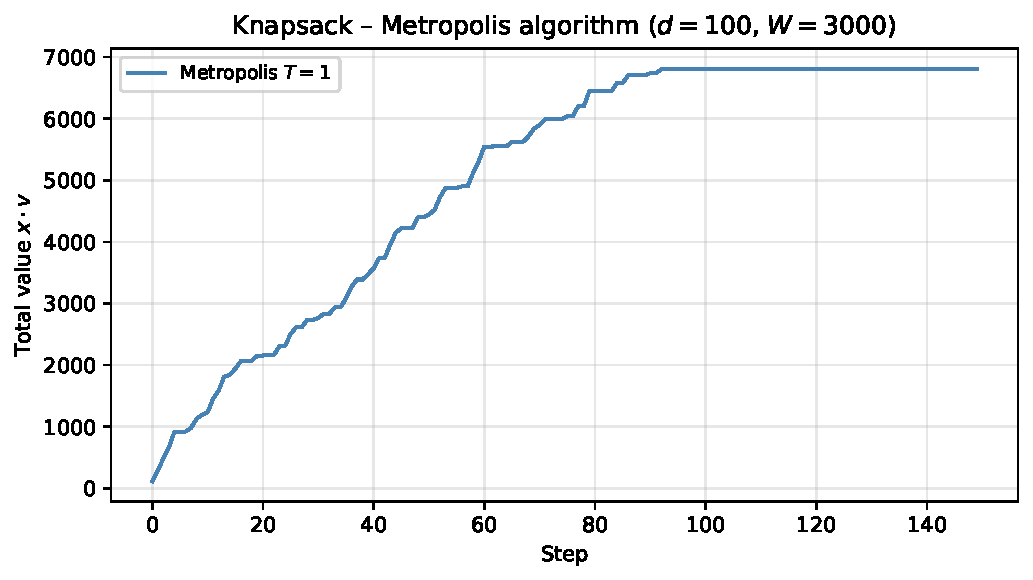
\includegraphics[width=\textwidth]{fig_lip_knapsack}
    \column{0.48\textwidth}
    \small
    \textbf{Knapsack ($d=100$, $M=100$ candidates):}\\
    LIP outperforms plain Metropolis -- informed proposals jump to
    higher-value neighbors.\\[6pt]

    \textbf{TSP (13 cities):}
    \begin{itemize}
      \item LIP ($M=100$): evaluates 100 of $\binom{13}{2}=78$ swaps
      \item Substantially faster convergence than plain Metropolis
      \item Winner in 9.66/100 runs vs.\ 0.33 for plain Metropolis
    \end{itemize}
    \vspace{4pt}
    \emph{Cost:} $\sim 100\times$ more expensive per step than Metropolis.
  \end{columns}
\end{frame}

% ============================================================
\section{7.4 Cross-Entropy Method}
% ============================================================

\begin{frame}{7.4 The Cross-Entropy Method -- Overview}
  \textbf{Different paradigm:}
  Instead of walking on the state space, \emph{update a family of
  distributions} $\{p_{\btheta}\}$ so that it concentrates near the optimum.

  \begin{block}{CE Optimization Setup (Eq.~7.4.1--7.4.2)}
    \begin{align*}
      s^{\mathrm{opt}} &= \arg\max_{s\in\calS} \pi_s = \arg\max_{s\in\calS} h(s),\\
      \gamma^{\mathrm{opt}} &= \max_{s\in\calS} h(s) \in \R.
    \end{align*}
    \begin{itemize}
      \item $h: \calS \to \R$ -- \textbf{performance function}
      \item $\{p_\theta : \theta \in \Theta\}$ -- parametric family (our choice)
      \item $\theta_0$ -- initial parameter (e.g.\ uniform)
    \end{itemize}
  \end{block}

  \textbf{Core idea:} relate the rare event
  $I(\gamma) = \Prob_{\theta_0}(h(\mathbf{X}) \ge \gamma)$
  (probability of being near-optimal) to the estimation problem, then
  update $\theta$ to make this event less rare.
\end{frame}

\begin{frame}{CE: Parametric Estimation Connection}
  Estimation problem:
  \[
    I(\gamma) = \Prob_{\theta_0}(h(\mathbf{X}) \ge \gamma)
    = \sum_{s \in \calS} \mathbf{1}(h(s) \ge \gamma)\, p_{\theta_0}(s)
    = \E_{\theta_0}\bigl[\mathbf{1}(h(\mathbf{X}) \ge \gamma)\bigr].
  \]
  If $\gamma = \gamma^{\mathrm{opt}}$ and $p_{\theta_0}$ is uniform:
  \[
    I(\gamma^{\mathrm{opt}}) = \frac{\#\{s : h(s) = \gamma^{\mathrm{opt}}\}}{|\calS|}
    \approx \frac{1}{|\calS|} \quad \text{(very small!)}.
  \]

  \textbf{CE strategy:} use IS-like parameter update to shift $\theta$ so
  that high-performance solutions are sampled more often.

  \medskip
  \begin{block}{CE Parameter Update (Eq.~7.4.5)}
    \[
      \theta' = \arg\max_\theta \frac{1}{M}
        \sum_{i:\, \mathbf{X}_i \in \mathcal{E}_t}
        \log p_\theta(\mathbf{X}_i),
    \]
    where \textbf{elite set} $\mathcal{E}_t = \{\mathbf{X}_i : h(\mathbf{X}_i) \ge \gamma_t\}$.
  \end{block}
\end{frame}

\begin{frame}{CE Method: Schematic}
  \begin{center}
    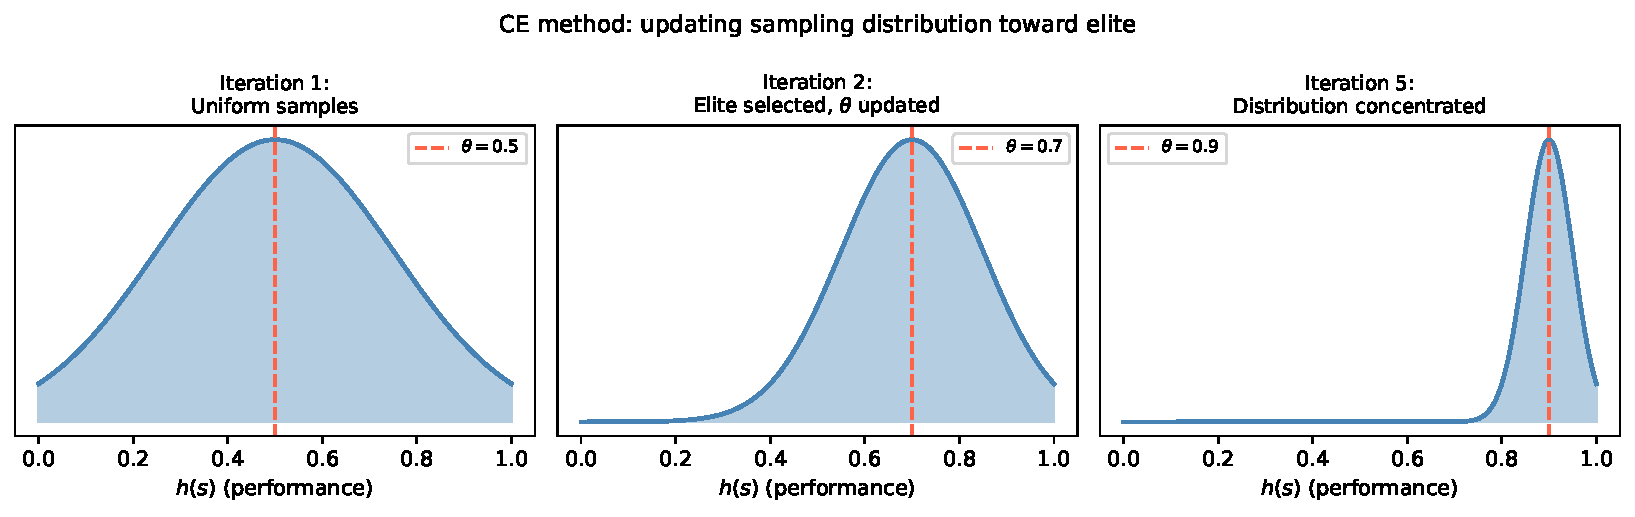
\includegraphics[width=0.90\textwidth]{fig_ce_schematic}
  \end{center}
  \small
  \textbf{Interpretation:} At each iteration, samples are drawn from
  current $p_\theta$. The top $(1-\rho)$ fraction (``elite'') are used
  to fit a new $\theta'$, shifting the distribution toward high-performance
  regions.
\end{frame}

\begin{frame}[allowframebreaks]{Algorithm 69: Cross-Entropy Method for Optimization}
  \textbf{Inputs:} family $\{p_\theta\}$, $\theta_0$, performance $h(\cdot)$,
  sample size $M$, elite fraction $\rho \in (0,1)$,
  smoothing $\alpha \in (0,1)$, stopping depth $d$ (default 5).

  \medskip
  \textbf{Repeat:} $t = 1, 2, \ldots$
  \begin{enumerate}
    \item \textbf{Update level $\gamma_t$:}
      Generate $\mathbf{X}_1,\ldots,\mathbf{X}_M \sim p_{\theta'_{t-1}}$.
      Sort performances $\eta_{(1)} \le \cdots \le \eta_{(M)}$.
      \[
        \gamma_t = \eta_{(\lceil(1-\rho)M\rceil)}.
      \]
    \item \textbf{Update parameter $\theta'_t$:} from the \emph{same} samples,
      let $\mathcal{E}_t = \{\mathbf{X}_i : h(\mathbf{X}_i) \ge \gamma_t\}$,
      \[
        \theta' = \arg\max_\theta \frac{1}{M} \sum_{i=1}^M \mathbf{1}(h(\mathbf{X}_i)\ge\gamma_t)
        \log p_\theta(\mathbf{X}_i).
      \]
      Apply \textbf{smoothed update:}
      \[
        \theta'_t = \alpha\,\theta' + (1-\alpha)\,\theta'_{t-1}.  \quad\text{(Eq.~7.4.6)}
      \]
  \end{enumerate}
  \textbf{Stop} when $\gamma_t = \gamma_{t-1} = \cdots = \gamma_{t-d}$.
  \textbf{Return} elite set $\mathcal{E}$.

  \framebreak
  \textbf{Differences from CE for estimation:}
  \begin{itemize}
    \item In estimation, $\theta_0$ is \emph{given}; in optimization,
      $\theta_0$ is our choice (e.g.\ uniform).
    \item No likelihood ratio / IS weights needed (Eq.~7.4.5 uses $W\equiv 1$).
    \item The level $\gamma_t$ \emph{increases} over iterations until it
      converges to $\gamma^{\mathrm{opt}}$.
    \item Output is the best \emph{solution} found, not an estimate.
  \end{itemize}
\end{frame}

\begin{frame}{CE for the 0-1 Knapsack Problem}
  \textbf{Parametric family:} independent Bernoulli coordinates,
  $\theta = (\theta_1,\ldots,\theta_d)$, $\theta_i \in [0,1]$.
  \[
    p_\theta(\bx) = \prod_{j=1}^d \theta_j^{x_j}(1-\theta_j)^{1-x_j}.
  \]
  Start with $\theta_0 = (1/2,\ldots,1/2)$ (uniform).

  \begin{block}{CE Update for Knapsack (Eq.~7.4.7)}
    \[
      \theta'_k
      = \frac{\displaystyle\sum_{i=1}^M \mathbf{1}(h(\mathbf{X}_i)\ge\gamma_t)\,\mathbf{X}_i}
             {\displaystyle\sum_{i=1}^M \mathbf{1}(h(\mathbf{X}_i)\ge\gamma_t)}.
    \]
    i.e.\ the \textbf{sample mean of elite solutions} -- a simple average!
  \end{block}

  The $k$-th coordinate of $\theta'$ is the fraction of elite samples
  that include item $k$.
\end{frame}

\begin{frame}[fragile]{CE Knapsack: Python Implementation}
  \begin{lstlisting}[style=python]
import numpy as np

def ce_knapsack(d, w, v, W, theta0, M=200, rho=0.1, alpha=0.7,
                d_stop=5, max_iter=50):
    theta = theta0.copy()
    gammas, best_vals = [], []
    gamma_history = []
    for t in range(max_iter):
        # Step 1: sample and compute performance
        X = (np.random.rand(M, d) < theta).astype(float)
        h = np.array([x @ v if x @ w <= W else 0.0 for x in X])
        # Step 2: compute elite level
        gamma_t = np.quantile(h, 1 - rho)
        gammas.append(gamma_t)
        # Step 3: elite update
        elite = h >= gamma_t
        if elite.sum() > 0:
            theta_new = X[elite].mean(axis=0)
            theta = alpha * theta_new + (1 - alpha) * theta
        best_vals.append(h.max())
        gamma_history.append(gamma_t)
        # Stopping criterion
        if (len(gamma_history) > d_stop and
                len(set(gamma_history[-d_stop:])) == 1):
            break
    return theta, best_vals, gammas
  \end{lstlisting}
\end{frame}

\begin{frame}{CE Convergence: Knapsack Results}
  \begin{center}
    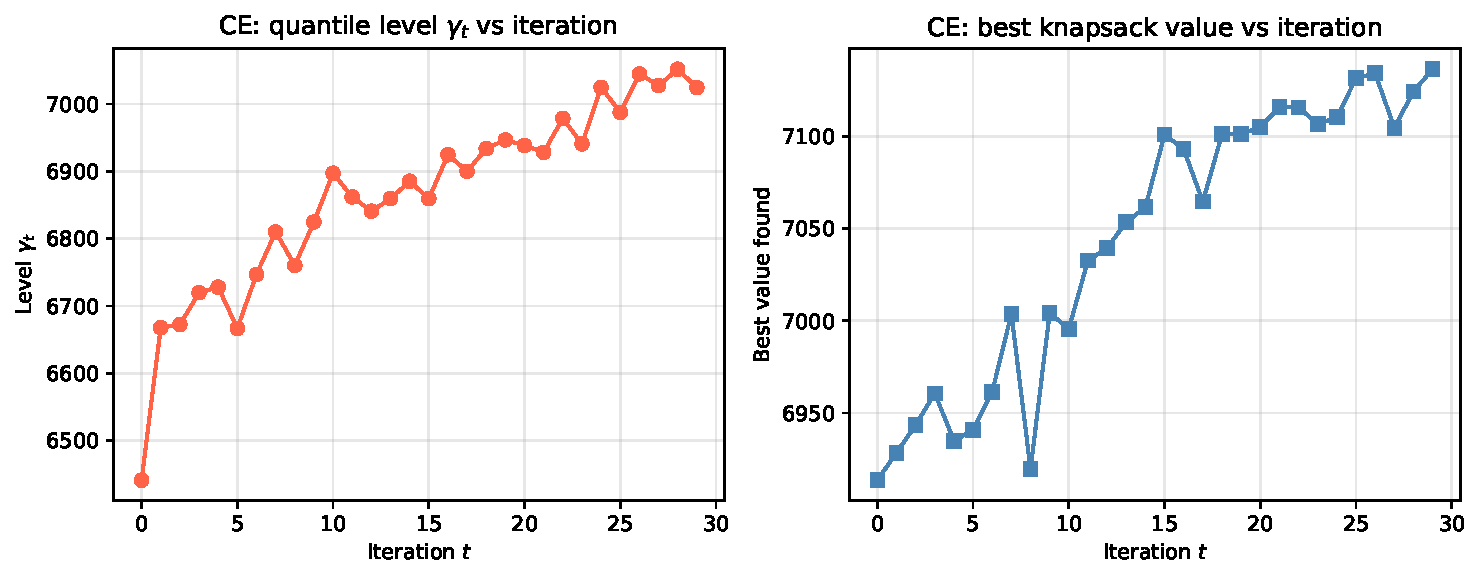
\includegraphics[width=0.82\textwidth]{fig_ce_convergence}
  \end{center}
  \small
  \textbf{Left:} the quantile level $\gamma_t$ increases monotonically,
  converging to $\gamma^{\mathrm{opt}}$.
  \textbf{Right:} best value found improves rapidly and plateaus.
  CE converges in $\sim 30$ iterations even for $d=100$.
\end{frame}

\begin{frame}{CE Parameter Evolution}
  \begin{columns}
    \column{0.55\textwidth}
    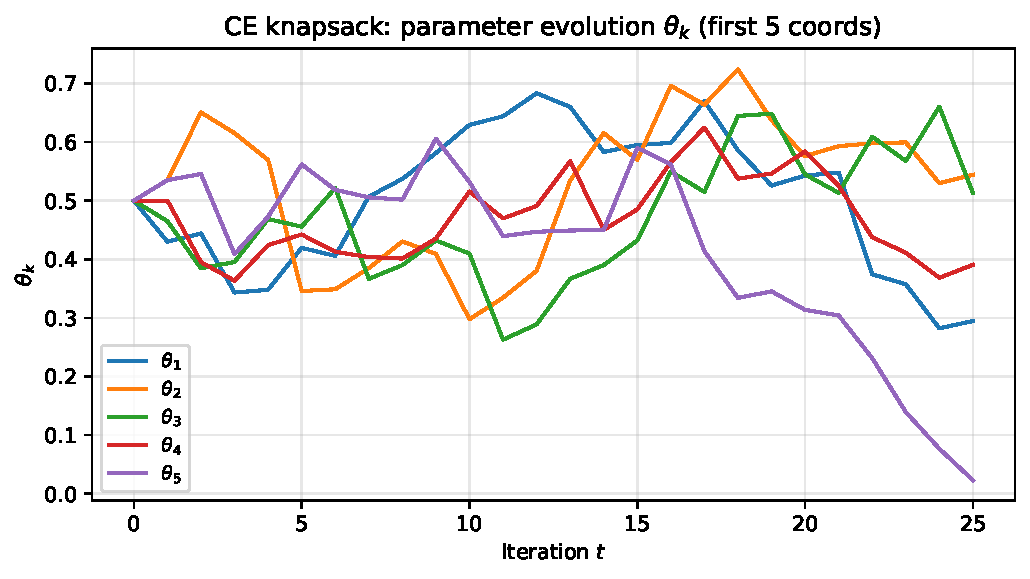
\includegraphics[width=\textwidth]{fig_ce_theta}
    \column{0.43\textwidth}
    \small
    Each $\theta_k$ converges to 0 or 1:\\[4pt]
    \begin{itemize}
      \item $\theta_k \to 1$: item $k$ is always in elite solutions
        (include it)
      \item $\theta_k \to 0$: item $k$ is never in elite solutions
        (exclude it)
    \end{itemize}
    \vspace{4pt}
    Items with high value-to-weight ratio converge to $\theta_k=1$ faster.\\[4pt]
    Smoothing parameter $\alpha$ prevents premature convergence.
  \end{columns}
\end{frame}

\begin{frame}{CE for the TSP: Parametric Family}
  \textbf{Parametric family for permutations:}
  $\theta = (\theta_{ij})$ -- a stochastic $n\times n$ matrix with
  $\theta_{ii} = 0$, $\theta_{ij} \ge 0$, $\sum_j \theta_{ij} = 1$.

  \begin{block}{Algorithm 70: Sample Permutation from $\theta$}
    \begin{enumerate}
      \item Set $\sigma_1 = 1$ (start city).
      \item For $k=1,\ldots,n-1$:
        \begin{itemize}
          \item Take row $k$ of $\theta$; zero out already-visited cities.
          \item Normalize remaining entries to get probability vector $\mathbf{q}^{k+1}$.
          \item Sample $\sigma_{k+1}$ from $\mathbf{q}^{k+1}$.
        \end{itemize}
    \end{enumerate}
  \end{block}

  \begin{block}{CE Update for TSP (Eq.~7.4.9)}
    \[
      \theta'_{ab}
      = \frac{\displaystyle\sum_{i=1}^M \mathbf{1}(h(\mathbf{X}_i)\ge\gamma_t)
               \sum_{k=1}^{n-1}\mathbf{1}(\sigma_k^{(i)}=a,\,\sigma_{k+1}^{(i)}=b)}
             {\displaystyle\lambda_a},
    \]
    where $\lambda_a$ is a normalising constant ensuring row sums equal 1.
  \end{block}
\end{frame}

\begin{frame}[fragile]{CE for TSP: Python Skeleton}
  \begin{lstlisting}[style=python]
import numpy as np

def sample_permutation(theta, n, rng):
    """Algorithm 70: sample a tour from stochastic matrix theta."""
    sigma = [0]   # start at city 0
    for k in range(n - 1):
        row = theta[sigma[-1]].copy()
        for already in sigma:
            row[already] = 0.0          # exclude visited
        row /= row.sum()                # normalise
        next_city = rng.choice(n, p=row)
        sigma.append(next_city)
    return sigma

def ce_tsp_update(elite_tours, n):
    """Compute theta' from elite tours (Eq. 7.4.9)."""
    counts = np.zeros((n, n))
    for tour in elite_tours:
        for k in range(len(tour) - 1):
            counts[tour[k], tour[k+1]] += 1
    # Normalise each row
    row_sums = counts.sum(axis=1, keepdims=True)
    row_sums[row_sums == 0] = 1
    return counts / row_sums
  \end{lstlisting}
\end{frame}

% ============================================================
\section{7.5 Metropolis Cross-Entropy: A Hybrid Approach}
% ============================================================

\begin{frame}{7.5 Metropolis--CE: A Hybrid Approach}
  \textbf{Metropolis:} random walk, state = current solution.\\
  \textbf{CE:} state = distribution $p_\theta$; $M$ solutions sampled each step.

  \medskip
  \textbf{Hybrid idea (Algorithm 72):} at each iteration,
  \begin{itemize}
    \item Generate $M$ \emph{neighbors} of $\mathbf{X}^{(t-1)}$ from the
      transition distribution $\mathbf{Q}_{\theta'_{t-1}}(\mathbf{X}^{(t-1)}, \cdot)$.
    \item Update $\theta$ as in CE using elite samples.
    \item Set next state $\mathbf{X}^{(t)}$ = best sample.
  \end{itemize}

  \begin{block}{Metropolis-CE Parameter Update (Eq.~7.5.1)}
    \[
      \theta' = \arg\max_\theta \frac{1}{M}
        \sum_{i=1}^M \mathbf{1}(h(\mathbf{X}_i) \ge \gamma_t)
        \log \mathbf{Q}_\theta(\mathbf{X}^{(t-1)}, \mathbf{X}_i).
    \]
    Smoothed: $\theta'_t = \alpha\,\theta' + (1-\alpha)\,\theta'_{t-1}$.
  \end{block}
\end{frame}

\begin{frame}{Metropolis-CE for Knapsack}
  \textbf{Distribution family:} $\theta = (\theta_1,\ldots,\theta_d)$,
  where $\sum_k \theta_k = 1$, $\theta_k \ge 0$.
  Neighbor $\mathbf{X}'$ is formed by picking coordinate $k$ to flip
  with probability $\theta_k$.

  \begin{block}{CE Update for Knapsack Neighbors (Eq.~7.5 detail)}
    \[
      \theta'_k = \frac{C_k}{\sum_{j=1}^d C_j}, \qquad
      C_k = \sum_{i=1}^M \mathbf{1}(h(\mathbf{X}_i) \ge \gamma_t).
    \]
    $C_k$ counts how often coordinate $k$ was flipped in elite samples.
  \end{block}

  \textbf{Result (100 runs):} Metropolis-CE \emph{always} wins among
  competing algorithms with $\rho=0.3$, $M=30$, $\alpha=0.001$,
  $T=100$ steps.
\end{frame}

\begin{frame}{Metropolis-CE for TSP}
  \textbf{Distribution family for swaps:}
  $\theta = (\theta(i,j))_{i<j}$, where $\theta(i,j)$ is the probability
  of swapping positions $i$ and $j$.

  \begin{block}{CE Update for TSP Swaps (Eq.~7.5.2)}
    \[
      \theta'(a,b)
      = \frac{C_{(a,b)}}{\displaystyle\sum_{i<j} C_{(i,j)}},
      \qquad
      C_{(a,b)} = \sum_{i=1}^M \mathbf{1}(h(\mathbf{X}_i)\ge\gamma_t)\,
        \mathbf{1}((a,b)\text{ swapped in }\mathbf{X}_i).
    \]
  \end{block}

  \textbf{Simulation ($M=100$, $\rho=0.35$, $\alpha=0.7$):}
  In 61 out of 100 runs the CE method (Alg.~71) won; in 29/100 runs
  Metropolis-CE won; LIP won 9.66/100 times.

  \begin{center}
    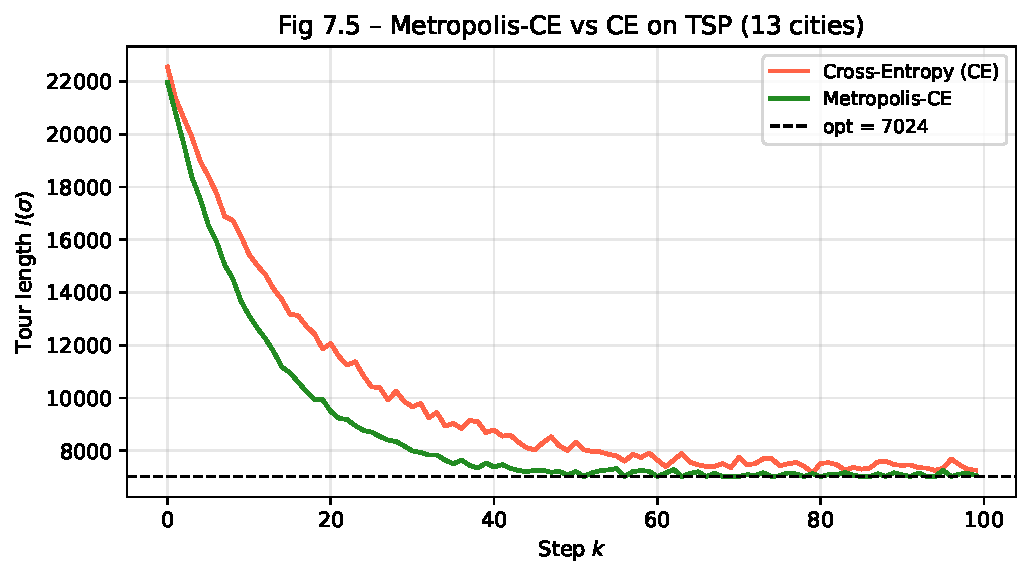
\includegraphics[width=0.50\textwidth]{fig_mce_vs_ce}
  \end{center}
\end{frame}

\begin{frame}[fragile]{Algorithm 72: Metropolis-CE (Python Sketch)}
  \begin{lstlisting}[style=python]
def metropolis_ce(x0, h, sample_neighbors, update_theta,
                  theta0, T=100, M=30, rho=0.3, alpha=0.001):
    """Metropolis-CE hybrid (Algorithm 72)."""
    theta = theta0.copy()
    X_cur = x0.copy()
    best = X_cur.copy()
    for t in range(1, T + 1):
        # Generate M neighbors of X_cur using distribution Q_theta
        Xs = [sample_neighbors(X_cur, theta) for _ in range(M)]
        perfs = np.array([h(X) for X in Xs])
        # Compute elite level
        gamma_t = np.quantile(perfs, 1 - rho)
        elite_mask = perfs >= gamma_t
        # Update theta from elite neighbors
        theta_new = update_theta(Xs, elite_mask, theta)
        theta = alpha * theta_new + (1 - alpha) * theta
        # Move to best sample
        best_idx = np.argmax(perfs)
        X_cur = Xs[best_idx]
        if h(X_cur) > h(best):
            best = X_cur.copy()
    return best
  \end{lstlisting}
\end{frame}

% ============================================================
\section{7.6 Summary: TSP and Knapsack Results}
% ============================================================

\begin{frame}{7.6 Summary of Simulation Results}
  \textbf{All algorithms run 100 times, each for a fixed number of steps.}

  \begin{block}{7.6.1 Travelling Salesman Problem (13 cities)}
    \begin{itemize}
      \item Optimal solution: \textbf{7024} (Held-Karp, $O(n^2 2^n)$ time)
      \item All experiments use distance matrix $\mathbf{M}$ from Fig.~7.3
    \end{itemize}
  \end{block}

  \begin{center}
    \small
    \begin{tabular}{lrrrr}
      \toprule
      Algorithm & Win score & Best (median) & Time (s) \\
      \midrule
      Metropolis ($T=1$)    & 0.33 & $\sim 8200$ & $<1$  \\
      SA ($T_k=1/\log k$)  & 0.00 & $\sim 7800$ & $<1$  \\
      LIP ($M=100$)         & 9.66 & $\sim 7500$ & $\sim 10$ \\
      Cross-Entropy         & 61.0 & $\sim 7300$ & $\sim 230$ \\
      Metropolis-CE         & 29.0 & $\sim 7050$ & $\sim 10$ \\
      \bottomrule
    \end{tabular}
  \end{center}
  \small
  CE wins most often on TSP; Metropolis-CE is a faster alternative.
\end{frame}

\begin{frame}{TSP Results: Visual Comparison}
  \begin{columns}
    \column{0.58\textwidth}
    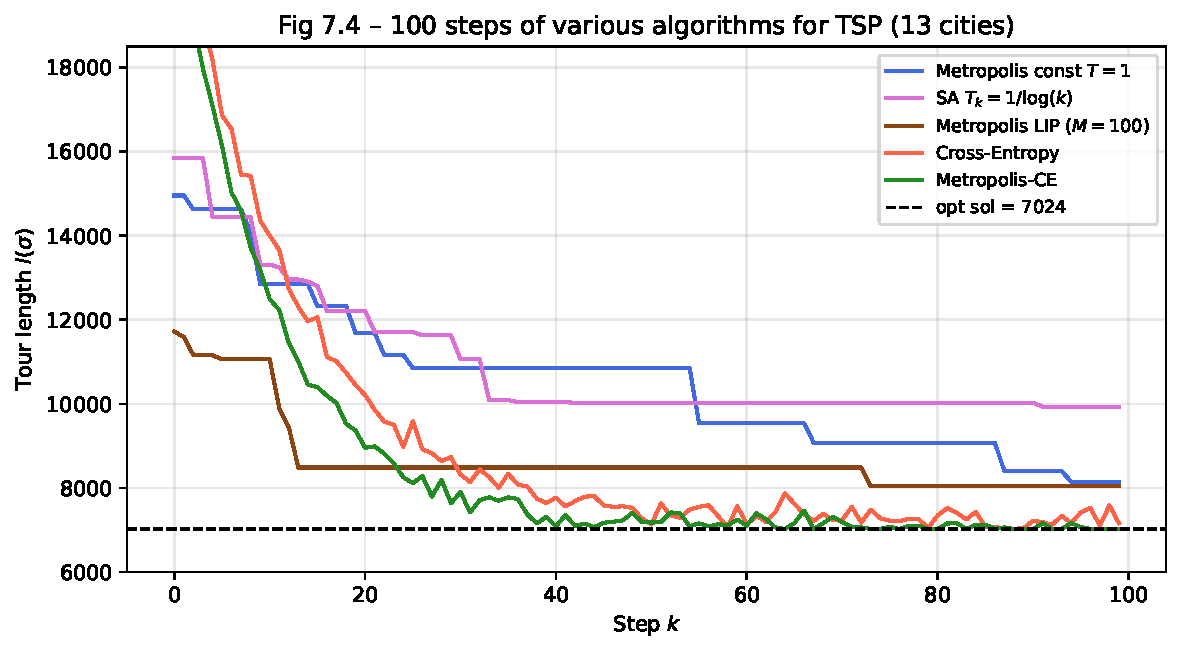
\includegraphics[width=\textwidth]{fig_tsp_comparison}
    \column{0.40\textwidth}
    \small
    \textbf{Key observations:}\\[4pt]
    \begin{itemize}
      \item Plain Metropolis ($T=1$) gets trapped at high tour lengths
      \item SA improves more quickly early on
      \item CE and Metropolis-CE converge fastest to near-optimal
      \item LIP provides good improvement at moderate cost
    \end{itemize}
    \vspace{4pt}
    Dashed line: optimal = 7024.
  \end{columns}
\end{frame}

\begin{frame}{Algorithm Comparison: Win Scores}
  \begin{center}
    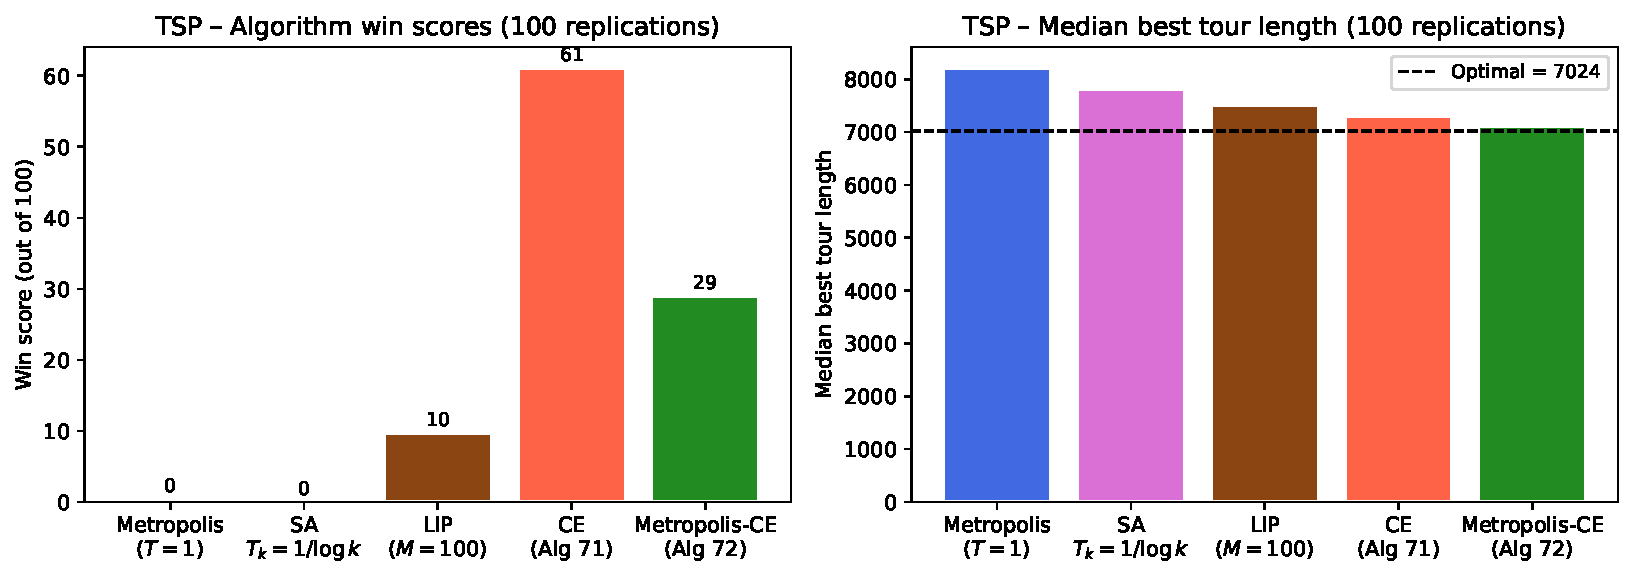
\includegraphics[width=0.82\textwidth]{fig_tsp_results_bar}
  \end{center}
  \small
  \textbf{Win score} = fraction of 100 replications where an algorithm
  found the best tour length.  CE-based methods dominate for TSP.
\end{frame}

\begin{frame}{7.6.2 Knapsack Problem Results}
  \textbf{Setup:} $d=100$, $w_i=i$, $v_i=i^{1.2}$, $W=3000$.

  \begin{block}{Summary Table 7.3 (100 replications)}
    \small
    \begin{tabular}{lrr}
      \toprule
      Algorithm & Best value (median) & Win score \\
      \midrule
      Metropolis ($T=1$)       & $\sim 6800$ & low \\
      Gibbs sampler ($T=1$)    & $\sim 6800$ & low \\
      Metropolis LIP           & $\sim 7100$ & moderate \\
      Cross-Entropy            & $\sim 7200$ & high \\
      Metropolis-CE            & $\sim 7400$ & \textbf{highest} \\
      \bottomrule
    \end{tabular}
  \end{block}

  \medskip
  \textbf{Observations:}
  \begin{itemize}
    \item Metropolis-CE always wins for knapsack in 100-step experiments
    \item CE and LIP both superior to uninformed Metropolis
    \item For knapsack the optimal value is not known (NP-hard), but
      CE-based methods reliably reach $\bv\cdot\bx \approx 7400$
  \end{itemize}
\end{frame}

% ============================================================
\section{7.7 Bibliographical Notes}
% ============================================================

\begin{frame}{7.7 Bibliographical Notes}
  \begin{itemize}
    \item \textbf{Metropolis for decryption:}
      Diaconis [24] -- early application of MCMC to code-breaking.
    \item \textbf{Simulated Annealing:}
      Hajek [76] proved convergence under logarithmic cooling.
      Kirk\-patrick, Gelatt, Vecchi (1983) introduced SA for combinatorial
      optimisation.
    \item \textbf{Locally Informed Proposals:}
      Grathwohl et al.\ [71] ``Oops I took a gradient: Scalable sampling
      for discrete distributions'' -- gradient-based approximations to LIP.
    \item \textbf{Cross-Entropy method:}
      Rubinstein \& Kroese [31] -- comprehensive reference.
      FACE algorithm = fully automated cross-entropy [31, Alg.~4.1].
    \item \textbf{TSP:}
      Held-Karp algorithm [82] optimal solution in $O(n^2 2^n)$.
      Optimal for 13-city instance found in 0.068 s.
    \item Convergence theory of non-homogeneous Markov chains follows from
      Proposition 6.3.2 (MH stationarity).
  \end{itemize}
\end{frame}

% ============================================================
\section{7.8 Exercises}
% ============================================================

\begin{frame}[allowframebreaks]{7.8 Selected Exercises}
  \begin{block}{Exercise 7.L.1 (Substitution Cipher)}
    Implement the Metropolis-based decryption algorithm.
    There are several helper files:
    \texttt{ch7\_cipher\_*}.
    Run for 3000 steps starting from a random permutation.
    Report the evolution of log-likelihood and the final decrypted message.
  \end{block}

  \begin{block}{Exercise 7.L.2 (Permutation Distribution)}
    Consider $\pi_\sigma = \frac{1}{z}\lambda^{d(\sigma,\sigma_{\mathrm{id}})}$,
    $\lambda > 0$, where $d(\sigma,\sigma') = \frac{1}{n}\sum_i |\sigma(i)-\sigma'(i)|$.
    \begin{enumerate}[(a)]
      \item Implement the Metropolis algorithm for this distribution using
        the TSP proposal (Algorithm 66). For which $\lambda$ is it applicable?
      \item Repeat with the Kendall $\tau$ distance.
      \item Use the 2-opt proposal (Remark 7.2.4) and compare.
    \end{enumerate}
  \end{block}

  \framebreak

  \begin{block}{Exercise 7.L.4 (Knapsack, Smaller Capacities)}
    Re-implement the Gibbs sampler for knapsack with $W \in \{50, 500, 1000, 3000\}$.
    Compare with random sampling.
  \end{block}

  \begin{block}{Exercise 7.L.5 (SA for Knapsack)}
    Construct a simulated annealing version of the knapsack Gibbs sampler
    with $\pi^{T_k}_{\bx} = \exp(\bv\cdot\bx/T_k)/z_{T_k}$ for $\bw\cdot\bx \le W$.
    Compare:
    \begin{itemize}
      \item Fixed $T_k=1$ (no annealing)
      \item Logarithmic $T_k = 1/\log(k)$
    \end{itemize}
    for $W=3000$ and $W=50$.
  \end{block}

  \begin{block}{Exercise 7.L.6 (CE for TSP, Alternative Parametrisation)}
    Implement CE for TSP with a vector $\theta = (\theta_1,\ldots,\theta_n)$
    over cities (instead of a stochastic matrix).
    Compare convergence speed and solution quality with the matrix
    parametrisation.
  \end{block}
\end{frame}

% ============================================================
\section{Summary}
% ============================================================

\begin{frame}{Chapter 7 Summary}
  \begin{block}{Five Stochastic Optimization Methods}
    \small
    \begin{tabular}{llll}
      \toprule
      Method & State & Key idea & Tuning \\
      \midrule
      Metropolis ($T$ fixed) & solution & Boltzmann dist.\ & $T$, graph \\
      Simulated Annealing & solution & decrease $T_k$ & cooling schedule \\
      Locally Informed & solution & informed proposal & $\beta$, $g(\cdot)$ \\
      Cross-Entropy & distribution $\theta$ & update elite & $M$, $\rho$, $\alpha$ \\
      Metropolis-CE & sol.\ + dist.\ & hybrid walk & all of above \\
      \bottomrule
    \end{tabular}
  \end{block}

  \medskip
  \textbf{Key takeaways:}
  \begin{itemize}
    \item All methods use the Boltzmann distribution as a bridge between
      probability and optimisation.
    \item Simulated annealing converges to the global optimum if cooling
      is slow enough ($\sum e^{-c/T_j} = \infty$).
    \item CE-based methods often outperform Metropolis-based ones on
      combinatorial problems (TSP, knapsack).
    \item Metropolis-CE combines best of both: cheap per-step cost with
      CE-quality guidance.
    \item Choice of method depends on problem size, computational budget,
      and available gradient/structure information.
  \end{itemize}
\end{frame}

\begin{frame}{Comparison: All Algorithms on TSP}
  \begin{center}
    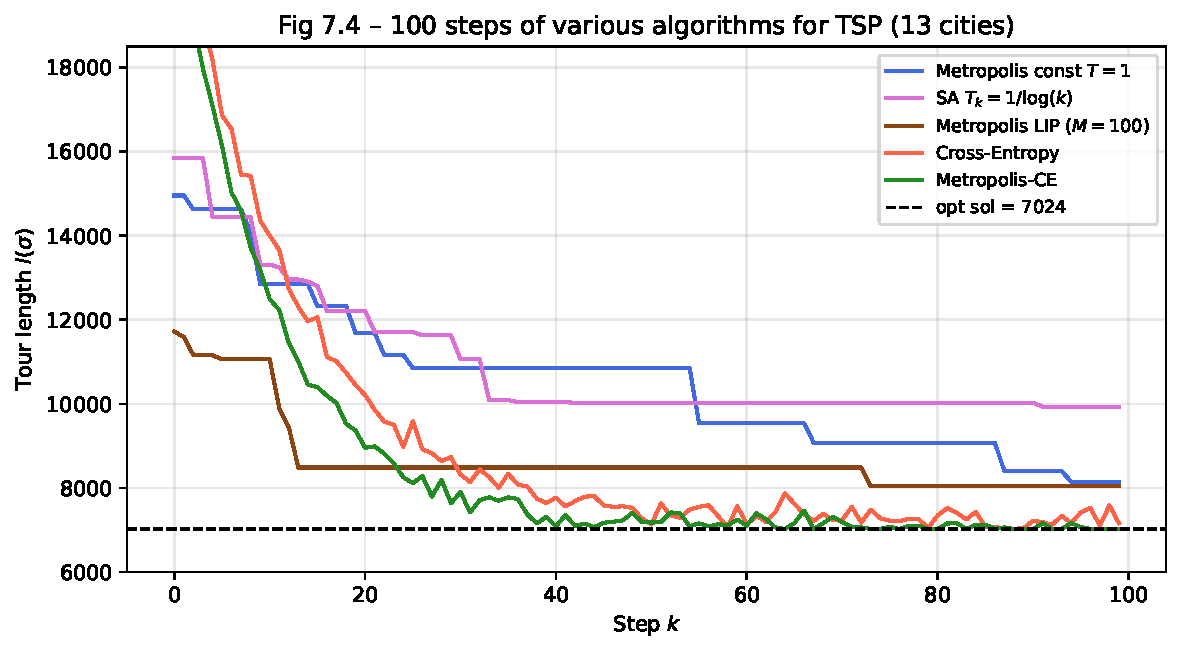
\includegraphics[width=0.60\textwidth]{fig_tsp_comparison}
  \end{center}
  \small
  \begin{center}
    \begin{tabular}{lc}
      \toprule
      Method & Character \\
      \midrule
      Metropolis (const.\ $T$) & Random walk, can get trapped \\
      Simulated Annealing & Escapes traps via high-$T$ phase \\
      LIP & Informed walk, moderate cost \\
      Cross-Entropy & Distribution-level learning \\
      Metropolis-CE & Hybrid: best of both worlds \\
      \bottomrule
    \end{tabular}
  \end{center}
\end{frame}

\end{document}
